\documentclass{standalone}
\usepackage{tikz}

\begin{document}
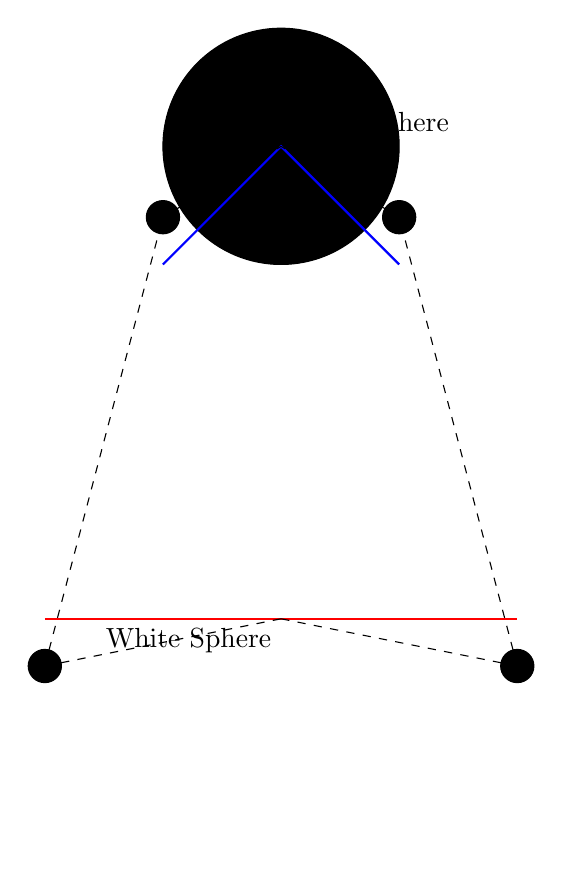
\begin{tikzpicture}[scale=3]
    % Draw the white sphere
    \filldraw[white] (0,0) circle (1cm);
    
    % Draw the black sphere at the top
    \filldraw[black] (0,2) circle (0.5cm);
    
    % Draw the red and blue strings
    \draw[red, thick] (-1,0) -- (0,0) -- (1,0);
    \draw[blue, thick] (-0.5,1.5) -- (0,2) -- (0.5,1.5);
    
    % Add connection points on the strings
    \filldraw[black] (-1,-0.2) circle (2pt);
    \filldraw[black] (1,-0.2) circle (2pt);
    \filldraw[black] (-0.5,1.7) circle (2pt);
    \filldraw[black] (0.5,1.7) circle (2pt);
    
    % Draw additional connections between points
    \draw[dashed] (-1,-0.2) -- (-0.5,1.7);
    \draw[dashed] (1,-0.2) -- (0.5,1.7);
    \draw[dashed] (-1,-0.2) -- (0,0);
    \draw[dashed] (1,-0.2) -- (0,0);
    \draw[dashed] (-0.5,1.7) -- (0,2);
    \draw[dashed] (0.5,1.7) -- (0,2);
    
    % Labeling the spheres
    \node[above right] at (0,2) {Black Sphere};
    \node[below left] at (0,0) {White Sphere};
\end{tikzpicture}
\end{document}